\chapter{Elemento Spring}

\section{Fundamento teórico}

El elemento \textit{Spring} (resorte) es un elemento finito unidimensional donde 
las coordenadas locales y globales coinciden. Cada elemento spring tiene dos 
nodos como se muestra en la figura \ref{fig:spring_element}. Sea la rigidez del 
resorte la denotada por $k$, en este caso la matriz de rigidez del elemento está 
dada por:

\begin{equation}
K_{(e)} = \begin{bmatrix}
k & -k \\
-k & k 
\end{bmatrix}
\end{equation}

\begin{center}
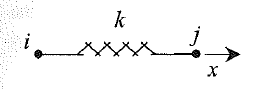
\includegraphics[scale=0.8]{src/spring-element/spring_element.png}
\captionof{figure}{Elemento spring}
\label{fig:spring_element}
\end{center}

Obviamente la matriz de rigidez para un elemento \textit{spring} es de $2\,x\,2$, dado que 
este tiene dos grados de libertada, uno en cada nodo. Consecuentemente para un 
sistema de elementos \textit{spring} con $n$ nodos, el tamaño de la matriz global de 
rigidez $K$ será de $n\,x\,n$. La matriz global de rigidez se obtiene ensamblando 
los matrices de rigidez por elemento $K_{(i)}$ para $i=1,2,...,n$, utilizando el método 
directo de la rigidez.\\

Una vez que la matriz global de rigidez $K$ es obtenida  se tiene un sistema de ecuaciones 
de la forma:

\begin{equation}
[K]\{U\} = \{F\}
\end{equation}

Donde $U$ es el vector global de desplazamientos nodales y $F$ es el vector global de 
fuerzas nodales.\\

El sistema de ecuaciones resultantes se puede simplificar aplicando las condiciones 
de frontera o restricciones de desplazamiento, quedando generalmente un sistema 
de menor dimensión el cuál está determinado y puede resolverse utilizando métodos 
de álgebra lineal´, quedando una posible solución como:

\begin{equation}
\overline{U} = \overline{K}^{-1}\, \overline{F}
\end{equation}

Donde $\overline{U}, \overline{K} \,\, y \,\, \overline{F}$ corresponden a las variables descritas 
anteriormente, después de aplicar las condiciones de frontera correspondientes.


\section{Un ejemplo resuelto en NuSA}

\textbf{Ejemplo 1.} Para el ensamble mostrado en la figura \ref{fig:example_01}, calcular 
a) la matriz global de rigidez  b) los desplazamientos de los nodos 3 y 4  c) las fuerzas 
de reacción en los nodos 1 y 2, y  d) las fuerzas en cada elemento. Una fuerza de 5000 lb 
es aplicada en el nodo 4 en la dirección $x$, las constantes de rigidez para cada resorte 
se muestran en la figura. Los nodos 1 y 2 están fijos. ~\cite{logan2007}

\begin{center}
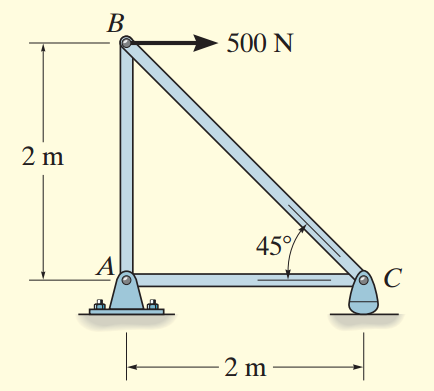
\includegraphics[scale=0.8]{src/spring-element/example_01.png}
\captionof{figure}{Ejemplo 1}
\label{fig:example_01}
\end{center}


Los pasos para solucionar el problema utilizando NuSA se resumen en la siguiente 
lista:

\begin{enumerate}
\item Importar las librerías a utilizar
\item Definir constantes o datos de entrada 
\item Crear un modelo del tipo correspondiente
\item Crear nodos y elementos
\item Agregar los nodos y elementos al modelo
\item Indicar las cargas y condiciones de frontera 
\item Resolver el modelo
\item Consultar los datos de salida requeridos
\end{enumerate}

Siguiendo la metodología anterior, vamos a ir \textit{desmenuzando} cada uno de los 
puntos expuestos.\\


\subsubsection*{Importar las librerías a utilizar}

Se importan los módulos \texttt{core}, \texttt{model} y \texttt{element}, que contienen 
todas las clases necesarias para crear y solucionar el modelo de elemento finito.

\begin{python}
from nusa.core import *
from nusa.model import *
from nusa.element import *
\end{python}


\subsubsection*{Definir constantes o datos de entrada}

En esta paso se crean variables con datos a utilizar en el resto del procedimiento, las 
cuales pueden ser fuerzas nodales aplicadas, desplazamientos preescritos, o bien constantes 
mecánicas del material.\\

Para nuestro ejemplo se definen la fuerza $P$ aplicada en el nodo 4 y las constantes de rigidez 
para cada resorte.

\begin{python}
# Definiendo constantes
P = 5000.0
k1, k2, k3 = 1000, 2000, 3000
\end{python}

\subsubsection*{Crear un modelo de tipo correspondiente}

Para este caso se crea un modelo instanciando un objeto de la clase \textit{SpringModel}.

\begin{python}
    m1 = SpringModel("2D Model")
\end{python}

Como puede notarse, el único argumento de entrada es un nombre para el modelo, mismo que no es necesario.


\subsubsection*{Crear nodos y elementos}



\begin{python}
# Nodos
n1 = Node((0,0))
n2 = Node((0,0))
n3 = Node((0,0))
n4 = Node((0,0))
# Elementos
e1 = Spring((n1,n3),k1)
e2 = Spring((n3,n4),k2)
e3 = Spring((n4,n2),k3)
\end{python}


\subsubsection*{Agregar los nodos y elementos al modelo}

\begin{python}
    for nd in (n1,n2,n3,n4):
        m1.addNode(nd)
    for el in (e1,e2,e3):
        m1.addElement(el)
\end{python}

\subsubsection*{Indicar las cargas y condiciones de frontera}

\begin{python}
    m1.addForce(n4,(P,))
    m1.addConstraint(n1,ux=0)
    m1.addConstraint(n2,ux=0)
\end{python}

\subsubsection*{Resolver el modelo}

\begin{python}
    m1.solve()
\end{python}


\subsubsection*{Consultar los datos de salida requeridos}

Se puede hacer una

\begin{python}
# a) Matriz global
print "a) Matriz global:\n {0}".format(m1.KG)
# b) Desplazamiento en los nodos 3 y 4
print "\nb) Desplazamientos de nodos 3 y 4"
print "UX3: {0}".format(n3.ux)
print "UX4: {0}".format(n4.ux)
# c) Fuerzas de reacción en los nodos 1 y 2
print "\nc) Fuerzas nodales en 1 y 2"
print "FX1: {0}".format(n1.fx)
print "FX2: {0}".format(n2.fx)
# d) Fuerzas en cada resorte
print "\nd) Fuerzas en elementos"
print "FE1:\n {0}".format(e1.fx)
print "FE2:\n {0}".format(e2.fx)
print "FE3:\n {0}".format(e3.fx)
\end{python}


\subsubsection*{All}

Ejecutando el script resultante:

\begin{python}
"""
Logan, D. (2007). A first course in the finite element analysis.
Example 2.1, pp. 42.
"""
P = 5000.0
k1, k2, k3 = 1000, 2000, 3000
# Model
m1 = SpringModel("2D Model")
# Nodes
n1 = Node((0,0))
n2 = Node((0,0))
n3 = Node((0,0))
n4 = Node((0,0))
# Elements
e1 = Spring((n1,n3),k1)
e2 = Spring((n3,n4),k2)
e3 = Spring((n4,n2),k3)

# Add elements 
for nd in (n1,n2,n3,n4):
    m1.addNode(nd)
for el in (e1,e2,e3):
    m1.addElement(el)

m1.addForce(n4,(P,))
m1.addConstraint(n1,ux=0)
m1.addConstraint(n2,ux=0)
m1.solve()

# a) Matriz global
print "a) Matriz global:\n {0}".format(m1.KG)
# b) Desplazamiento en los nodos 3 y 4
print "\nb) Desplazamientos de nodos 3 y 4"
print "UX3: {0}".format(n3.ux)
print "UX4: {0}".format(n4.ux)
# c) Fuerzas de reacción en los nodos 1 y 2
print "\nc) Fuerzas nodales en 1 y 2"
print "FX1: {0}".format(n1.fx)
print "FX2: {0}".format(n2.fx)
# d) Fuerzas en cada resorte
print "\nd) Fuerzas en elementos"
print "FE1:\n {0}".format(e1.fx)
print "FE2:\n {0}".format(e2.fx)
print "FE3:\n {0}".format(e3.fx)
\end{python}


Nos arroja como salida en consola los datos consutados:

\begin{verbatim}
NuSA 0.1.0
__________

a) Matriz global:
 [[ 1000.     0. -1000.     0.]
 [    0.  3000.     0. -3000.]
 [-1000.     0.  3000. -2000.]
 [    0. -3000. -2000.  5000.]]

b) Desplazamientos de nodos 3 y 4
UX3: 0.909090909091
UX4: 1.36363636364

c) Fuerzas nodales en 1 y 2
FX1: -909.090909091
FX2: -4090.90909091

d) Fuerzas en elementos
FE1:
 [[-909.09090909]
 [ 909.09090909]]
FE2:
 [[-909.09090909]
 [ 909.09090909]]
FE3:
 [[ 4090.90909091]
 [-4090.90909091]]
\end{verbatim}